\chapter{Phase 0 --- Préparation des données}

\section{Objectifs}

\begin{itemize}[nosep]
    \item Rééchantillonnage des séries à \texttt{PixelSpacing} incohérent (\S\ref{sec:bug-ordre-frames} du chapitre précédent).
    \item Normalisation des noms de segments (casse, alias).
    \item Correction N4 uniforme sur les 56 séries (voir \S\ref{sec:n4-manquant}).
    \item Construction du jeu de données (image, masque) aligné et consolidé via \texttt{load\_aligned\_pair}.
    \item Exclusion des 5 séries à géométrie non résolue tant qu'elles ne sont pas vérifiées manuellement.
    \item Définition d'un split train/val/test au niveau patient (14 patients).
\end{itemize}

\section{Vue d'ensemble du pipeline implémenté}

Quatre modules ont été écrits, chacun correspondant à une décision distincte pour pouvoir la
justifier et la tester séparément :

\begin{center}
\begin{tabular}{ll}
\toprule
Fichier & Rôle \\
\midrule
\texttt{src/data\_loading.py} & Chargement aligné (frame $\leftrightarrow$ slice, transposition H/W, résolution par nom) \\
\texttt{src/preprocessing.py} & \texttt{n4\_bias\_correction}, \texttt{resample\_volume\_and\_mask}, \texttt{normalize\_volume} \\
\texttt{scripts/build\_dataset.py} & Exécute le pipeline complet sur les 56 séries, écrit le dataset consolidé \\
\texttt{scripts/make\_split.py} & Split train/val/test au niveau patient \\
\texttt{scripts/validate\_normalization.py} & Validation empirique (CNR brut vs N4 vs normalisé) \\
\bottomrule
\end{tabular}
\end{center}

\texttt{src/data\_loading.py} reprend telle quelle la logique validée pendant l'EDA
(chapitre~\ref{chap:exploration}) --- aucune décision nouvelle ici, seulement une
consolidation du code déjà testé sur les 56 séries.

L'ordre du pipeline par série est : \textbf{chargement aligné} (DICOM brut, jamais les
anciens \texttt{volume\_n4.npy} archivés, \S\ref{sec:n4-manquant}) $\to$ \textbf{N4}
$\to$ \textbf{rééchantillonnage si nécessaire} $\to$ \textbf{normalisation
d'intensité}. N4 est appliqué avant le rééchantillonnage pour estimer le champ de biais
à une résolution la plus proche possible de l'acquisition d'origine.

\section{Rééchantillonnage}

\subsection{Décision}

Cible : \textbf{1,0\,mm}, la résolution de 51 des 56 séries (\S\ref{sec:bug-ordre-frames}).
Interpolation \textbf{linéaire} pour l'image, \textbf{plus-proche-voisin} pour le masque
--- une interpolation continue sur des labels entiers créerait des valeurs de classe
inexistantes aux frontières entre structures. L'axe temporel (les 20 frames) n'est
jamais rééchantillonné, seuls les deux axes spatiaux H/W le sont.

\textbf{Justification (littérature)} : reprend le concept de \emph{target spacing} de
nnU-Net (Isensee et al., 2021, \emph{Nature Methods}) --- rééchantillonner tous les cas
vers un spacing commun (ici, le spacing majoritaire du dataset) pour que les filtres
convolutifs voient une échelle physique cohérente d'une série à l'autre. Sans ça, une
même structure anatomique occuperait un nombre de pixels différent selon la série
d'origine, ce qui biaiserait l'apprentissage de features à une échelle donnée.

\subsection{Résultat}

La fonction \texttt{resample\_volume\_and\_mask} a été testée isolément sur une série à
0,7812\,mm (\texttt{2017-110\_01-0223-V1MR/RSSFP D}, réinterprétée avec un spacing
simulé pour le test) : rééchantillonnage $320\times320 \to 250\times250$ px, cohérent
avec le ratio $0,7812/1,0$, et les 6 valeurs de classe sont toutes préservées dans le
masque rééchantillonné (pas de perte de structure par arrondi).

\textbf{Dans l'exécution réelle sur les 56 séries, aucune n'a été rééchantillonnée} : les
5 séries à spacing anormal sont exactement les 5 séries à géométrie non résolue
(\S\ref{sec:bug-ordre-frames}), donc déjà exclues du pipeline pour une autre raison. La
fonction reste nécessaire pour le jour où ces 5 séries seront vérifiées et
réintégrées.

\section{Correction du champ de biais (N4)}

\subsection{Décision}

\texttt{n4\_bias\_correction} (\texttt{src/preprocessing.py}) applique
\texttt{SimpleITK.N4BiasFieldCorrectionImageFilter} : champ de biais estimé sur une
version sous-échantillonnée (facteur 4, coût prohibitif en pleine résolution), puis
appliqué à l'image en pleine résolution.

\textbf{Justification (littérature, avec une réserve assumée)} : N4ITK (Tustison et
al., 2010, \emph{IEEE Transactions on Medical Imaging}) est la méthode de référence pour
corriger l'inhomogénéité de réception RF, un artefact d'acquisition et non un signal
biologique. \textbf{Réserve} : nnU-Net n'inclut pas N4 dans son pipeline automatique par
défaut --- ce n'est donc pas une pratique universellement validée pour maximiser la
performance brute d'un modèle de segmentation. La justification retenue ici est
\textbf{spécifique à ce projet}, pas une reprise d'un standard : l'objectif de la thèse
est l'interprétabilité (voir chapitre~\ref{chap:contexte}), et on veut éviter qu'un
artefact d'acquisition explique une partie de la saillance du modèle ou de l'écart
FLASH/RSSFP mesuré en EDA (\S\ref{sec:flash-vs-rssfp}) plutôt qu'un vrai raisonnement
anatomique.

Remarque de méthode notée dans le code (\texttt{src/preprocessing.py}) : les
``slices'' du pseudo-volume corrigé sont en réalité des frames temporelles d'une même
coupe anatomique (IRM dynamique), pas des coupes spatiales adjacentes. Traiter la pile
comme un volume 3D pour l'estimation du champ de biais reste néanmoins raisonnable
physiquement : le champ de biais dépend de la géométrie antenne/patient, qui varie peu
sur la durée de l'acquisition --- ce n'est pas un détournement de la méthode.

\subsection{Validation empirique}

Plutôt que de faire confiance à la justification théorique seule (leçon déjà tirée sur
ce projet, voir feedback méthodologique sur l'alignement image/masque), l'effet de N4
sur le CNR par structure a été mesuré directement (\texttt{scripts/validate\_normalization.py}),
sur 2 séries d'un même patient (\texttt{2017-110 01-0229-V1MR}, FLASH D et RSSFP D) :

\begin{center}
\begin{tabular}{llrr}
\toprule
Série & Structure & CNR brut & CNR après N4 \\
\midrule
FLASH D  & ASC  & 2,311 & 2,996 \\
FLASH D  & PB   & 0,577 & 0,824 \\
RSSFP D  & ASC  & 0,046 & 0,100 \\
RSSFP D  & PB   & 0,919 & 1,048 \\
\bottomrule
\end{tabular}
\end{center}

\textbf{Résultat notable} : sur ce cas de test, N4 \textbf{augmente} le CNR pour
\emph{toutes} les structures des deux séries (table complète dans
\texttt{report/figures/validation\_normalisation\_cnr.csv}), pas seulement le préserve.
Cohérent avec l'effet attendu : retirer une variation basse fréquence de l'intensité
réduit l'écart-type du fond, ce qui augmente mécaniquement le rapport contraste/bruit.
\textbf{Limite assumée} : validé sur 1 patient / 2 séries seulement --- un indice
favorable, pas une preuve généralisée sur les 56 séries.

\section{Normalisation d'intensité}
\label{sec:normalisation}

\subsection{Décision}

\texttt{normalize\_volume} : clip aux percentiles [0,5, 99,5] puis z-score, calculé
\textbf{par volume} (jamais de statistiques globales partagées entre séquences ou
patients).

\subsection{Justification, avec une correction assumée}

\textbf{Le z-score par cas est bien le défaut nnU-Net pour l'IRM} --- vérifié dans la
documentation officielle (\texttt{explanation\_normalization.md} du dépôt nnU-Net) :
contrairement au CT (où les unités Hounsfield sont physiquement standardisées, donc
nnU-Net utilise des statistiques globales), l'IRM n'a pas d'échelle d'intensité
universelle (gain récepteur, antenne, réglages scanner) --- chaque cas doit être
normalisé avec ses propres statistiques.

\textbf{Correction} : une version antérieure de ce document présentait le \emph{clip
percentile avant z-score} comme faisant lui-même partie de ce défaut nnU-Net pour
l'IRM. \textbf{C'est inexact} : chez nnU-Net, le clip percentile [0,5, 99,5] est
spécifique au schéma \emph{CT}, avec des percentiles calculés globalement sur tout le
dataset d'entraînement, pas par volume. Le clip ajouté ici est une
\textbf{adaptation motivée empiriquement}, pas une reprise du standard : l'EDA a
identifié un cas concret (le point hyperintense de flux vasculaire sur ASC en FLASH,
\S\ref{sec:flash-vs-rssfp}) qui, sans clip, gonflerait la moyenne/écart-type utilisées
pour le z-score et écraserait le contraste du reste de l'image.

\textbf{Pourquoi pas d'autres alternatives standard} :
\begin{itemize}[nosep]
    \item \emph{Histogram matching} (Nyúl \& Udupa, 1999, \emph{Magnetic Resonance in
        Medicine}, vol. 42) --- écarté volontairement : aligner les histogrammes de
        toutes les séries sur une référence commune effacerait activement la différence
        de contraste FLASH vs RSSFP que ce projet cherche justement à mesurer et
        expliquer (\S\ref{sec:flash-vs-rssfp}).
    \item Statistiques globales sur tout le dataset --- écarté car FLASH et RSSFP ont
        des paramètres d'acquisition différents (TR/TE/FlipAngle constants mais
        différents par séquence, \S\ref{chap:exploration}) donc des échelles
        d'intensité brute non comparables.
\end{itemize}

\subsection{Validation empirique}

Même script que pour N4, comparaison brut / après N4 / après N4 + normalisation :

\begin{center}
\begin{tabular}{llrrr}
\toprule
Série & Structure & CNR brut & Après N4 & Après N4 + normalisation \\
\midrule
FLASH D  & ASC  & 2,311 & 2,996 & 2,758 \\
FLASH D  & VSC  & 0,409 & 0,632 & 0,643 \\
RSSFP D  & ASC  & 0,046 & 0,100 & 0,104 \\
RSSFP D  & VSC  & 0,250 & 0,300 & 0,306 \\
\bottomrule
\end{tabular}
\end{center}

Le clip + z-score préserve globalement le CNR obtenu après N4 (écarts de quelques
centièmes), à l'exception d'ASC en FLASH qui redescend légèrement (2,996 $\to$ 2,758) ---
attendu et voulu : c'est justement la queue extrême de cette distribution (le pic de
flux) que le clip neutralise dans le calcul des statistiques, sans supprimer le
signal lui-même de l'image.

\begin{center}
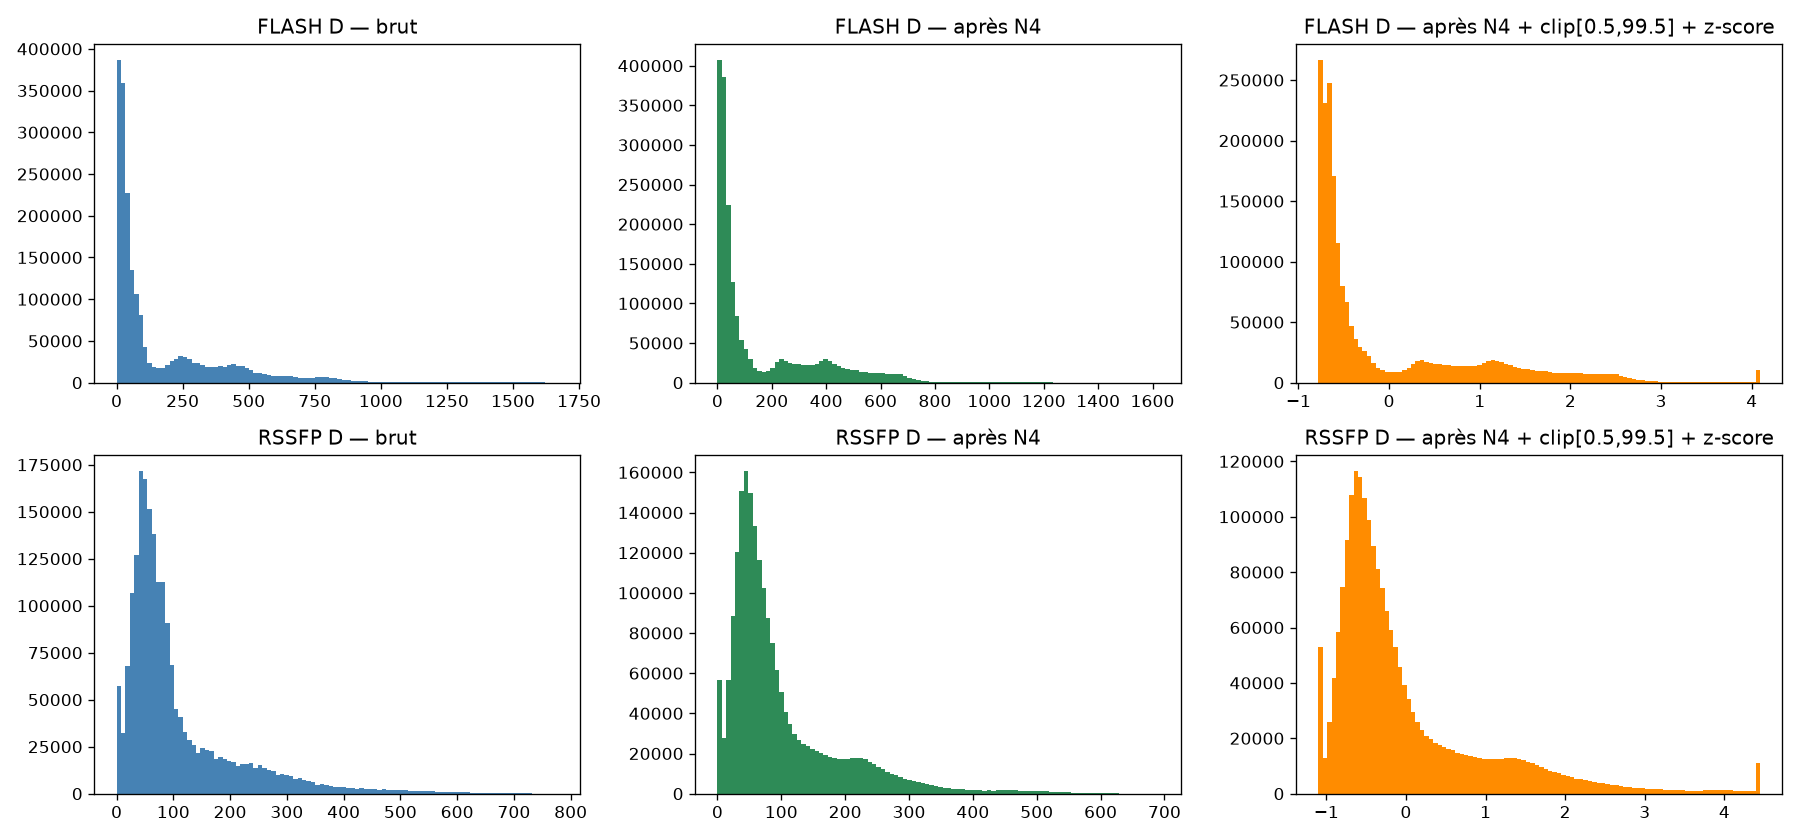
\includegraphics[width=\textwidth]{figures/validation_normalisation_hist.png}
\end{center}

Histogrammes d'intensité, FLASH D et RSSFP D du même patient, à chaque étape du
pipeline (brut / après N4 / après clip+z-score) --- la forme générale de la
distribution est préservée à chaque étape, seule l'échelle change, cohérent avec la
table de CNR ci-dessus.

\section{Résolution des structures par nom}

Reprend sans changement la logique validée en EDA (\S\ref{chap:exploration}) : chaque
structure est résolue par son nom d'en-tête (table d'alias \texttt{MCS}
$\to$ \texttt{MSC}, etc.), jamais par sa valeur de \texttt{LabelValue} brute --- l'EDA a
montré que PB est stockée sous 3 valeurs de label différentes (5, 6, 7) selon le
fichier.

\section{Exécution du pipeline complet}

\texttt{scripts/build\_dataset.py} exécuté sur les 56 séries :

\begin{itemize}[nosep]
    \item \textbf{51/56 séries traitées avec succès}, mêmes 5 exclues que dans l'EDA
        (géométrie non résolue).
    \item Temps de traitement : 0,3 à 1,3\,s par série (dominé par N4), quelques
        dizaines de secondes pour l'ensemble.
    \item Sortie : \texttt{DATA\_processed/<patient>/<série>/\{image.npy, label.npy\}}
        (image en \texttt{float32} normalisée, masque en \texttt{uint8} canonique
        1--6), $\approx$ 498\,Mo au total, plus un \texttt{manifest.csv} récapitulatif
        (statut, spacing d'origine, rééchantillonnage appliqué ou non, forme finale,
        temps de traitement).
    \item \texttt{2017-110\_01-0224-V1MR} (outlier de barycentre récurrent, \S
        \ref{sec:composantes-connexes}, jamais formellement vérifié sous 3D Slicer) est
        traitée normalement mais marquée \texttt{a\_verifier\_manuellement=True} dans
        le manifeste --- traçable sans bloquer le pipeline, en attendant la
        vérification.
\end{itemize}

\begin{center}
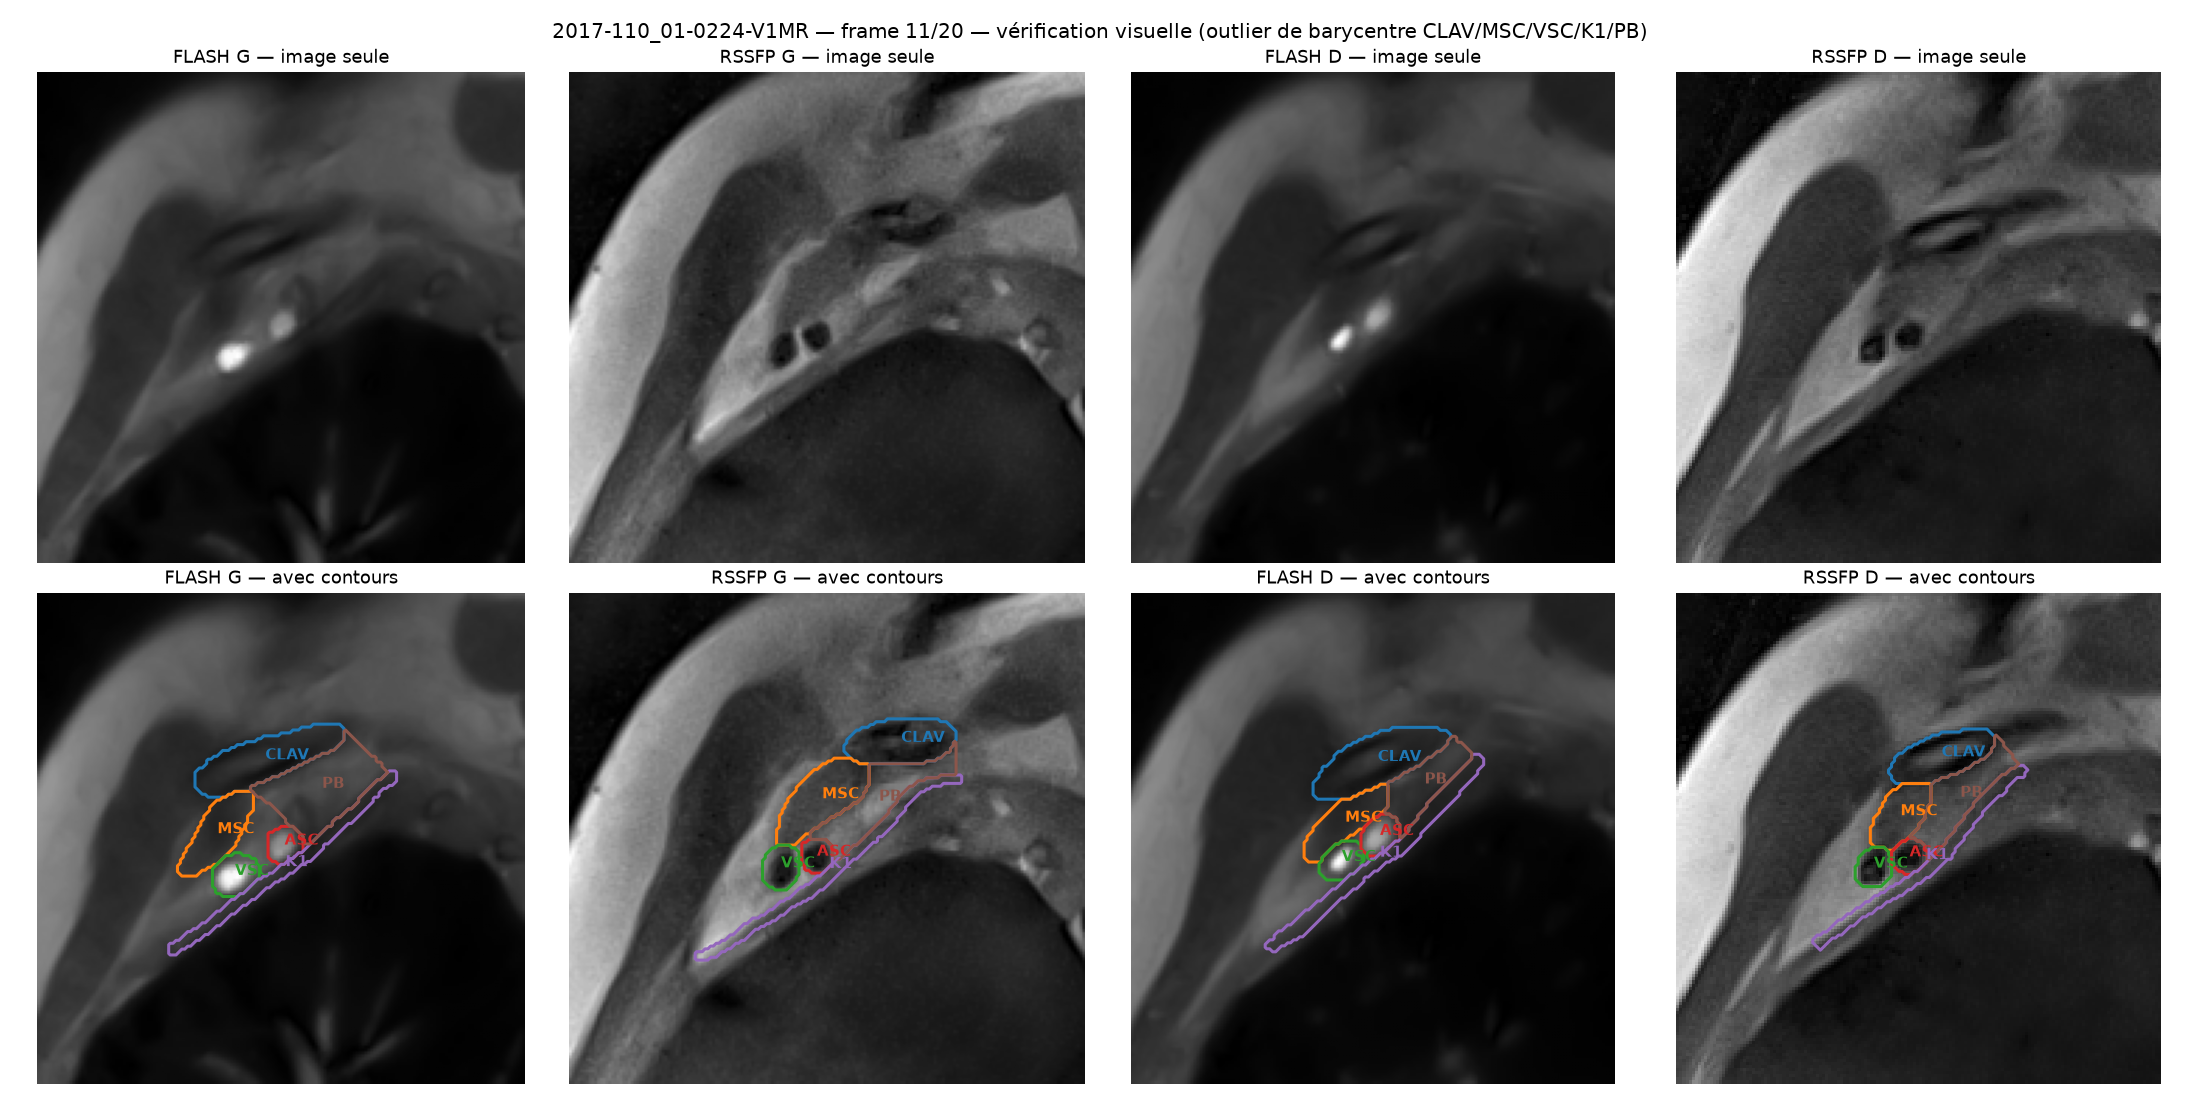
\includegraphics[width=\textwidth]{figures/verification_0224.png}
\end{center}

Vérification visuelle préliminaire (pas un substitut à 3D Slicer) sur ce patient : les
4 séries (FLASH/RSSFP D/G), une frame centrale, contours superposés. Rien ne saute aux
yeux comme clairement faux --- CLAV suit l'os incurvé, VSC/ASC sont bien positionnées
sur l'amas de vaisseaux, K1 trace une structure longue cohérente, et les 4 séries se
ressemblent entre elles. N'exclut pas une erreur subtile non visible sur cette seule
frame (1 sur 20) ; ne remplace pas la vérification manuelle complète sous 3D Slicer,
qui nécessite un jugement anatomique/clinique.

\section{Split train/val/test}

\subsection{Décision et bug de méthode corrigé}

Split au niveau \textbf{patient} (13 patients éligibles sur 14 --- \texttt{0222} est
entièrement exclu, 0 série utilisable), pour éviter toute fuite entre séries D/G ou
FLASH/RSSFP d'un même patient.

\textbf{Bug trouvé et corrigé pendant l'implémentation} : la première version du split
tirait les 13 patients éligibles au hasard sans distinguer ceux marqués
\texttt{a\_verifier\_manuellement} --- résultat, \texttt{2017-110\_01-0224-V1MR} est
tombé par hasard dans le split de \textbf{validation}. Risqué : si ses annotations
s'avèrent erronées lors de la vérification 3D Slicer, ça aurait faussé silencieusement
les métriques d'évaluation, pas seulement l'entraînement. \textbf{Corrigé} : tout
patient marqué \texttt{a\_verifier\_manuellement} est désormais forcé en train (impact
dilué sur beaucoup de cas) et ne peut jamais tomber en val/test tant qu'il n'est pas
confirmé.

\textbf{Justification (littérature)} : Varoquaux \& Cheplygina (2022, \emph{npj Digital
Medicine}, ``Machine learning for medical imaging: methodological failures and
recommendations'') identifient la fuite de données au niveau patient et l'absence de
curation des cas atypiques avant entraînement comme deux des causes les plus
fréquentes de sur-estimation de performance en imagerie médicale --- les deux
préoccupations traitées ici.

\subsection{Résultat (graine 42)}

\begin{center}
\begin{tabular}{ll}
\toprule
Split & Patients \\
\midrule
Train (9) & 0224, 0226, 0227, 0228, 0229, 0230, 0236, 0237, 0241 \\
Val (2)   & 0223, 0231 \\
Test (2)  & 0240, 0242 \\
\bottomrule
\end{tabular}
\end{center}

(\texttt{2017-110\_01-0222-V1MR} exclu, 0 série utilisable ; identifiants patient
abrégés au numéro final.)

\subsection{Point résolu en Phase 1}

Avec seulement 13 patients éligibles, un split fixe laisse très peu de patients en
val/test (2 chacun) --- l'évaluation sur un split aussi petit serait bruitée, une
variation d'un seul patient pouvant faire basculer une métrique de façon importante.
\textbf{Décision prise en Phase 1} (chapitre Protocole expérimental) : abandon du
split fixe au profit d'une validation croisée \texttt{KFold} au niveau patient
($k=3$) --- chaque patient passe exactement une fois en validation, et la comparaison
FLASH vs RSSFP est faite au niveau patient plutôt qu'au niveau fold pour rester
statistiquement exploitable malgré le petit $k$ (voir justification détaillée dans
le chapitre Protocole expérimental).

Reste ouvert, non tranché avec l'encadrant : si D et G doivent être traités comme un
flip horizontal l'un de l'autre --- en attendant, le flip horizontal n'est pas utilisé
comme augmentation (choix conservateur, voir chapitre Méthodologie).

\section{Sources et justifications --- récapitulatif}

\begin{center}
\begin{tabular}{lp{9cm}}
\toprule
Décision & Source \\
\midrule
Rééchantillonnage vers un spacing cible & nnU-Net, Isensee et al. (2021), \emph{Nature Methods} \\
Correction N4 & N4ITK, Tustison et al. (2010), \emph{IEEE TMI} --- justification spécifique au projet (interprétabilité), pas une reprise de la pratique nnU-Net par défaut \\
Z-score par cas (IRM) & nnU-Net (défaut confirmé dans la documentation officielle du dépôt) \\
Clip percentile avant z-score & Adaptation empirique motivée par l'EDA, pas un défaut nnU-Net \\
Histogram matching (écarté) & Nyúl \& Udupa (1999), \emph{Magnetic Resonance in Medicine} \\
Split patient-level, exclusion des cas non vérifiés & Varoquaux \& Cheplygina (2022), \emph{npj Digital Medicine} \\
\bottomrule
\end{tabular}
\end{center}

\todonote{Vérification manuelle encore en attente (non bloquante pour la Phase 1,
ces séries restent exclues) : les 6 séries non résolues
(\texttt{0222} $\times$4, \texttt{0223/FLASH D}, \texttt{0224} $\times$4).}
